% CodeMixESC pipeline (compile: pdflatex pipeline.tex -> pipeline.pdf, used by main.tex)
\documentclass[tikz,border=4pt]{standalone}
\usepackage[T1]{fontenc}
\usepackage{helvet}
\renewcommand{\familydefault}{\sfdefault}
\usetikzlibrary{arrows.meta,fit,backgrounds,calc}
\definecolor{orig}{HTML}{DBE8FB}
\definecolor{origline}{HTML}{3B6FB6}
\definecolor{new}{HTML}{FDE3C8}
\definecolor{newline}{HTML}{E8710A}
\begin{document}
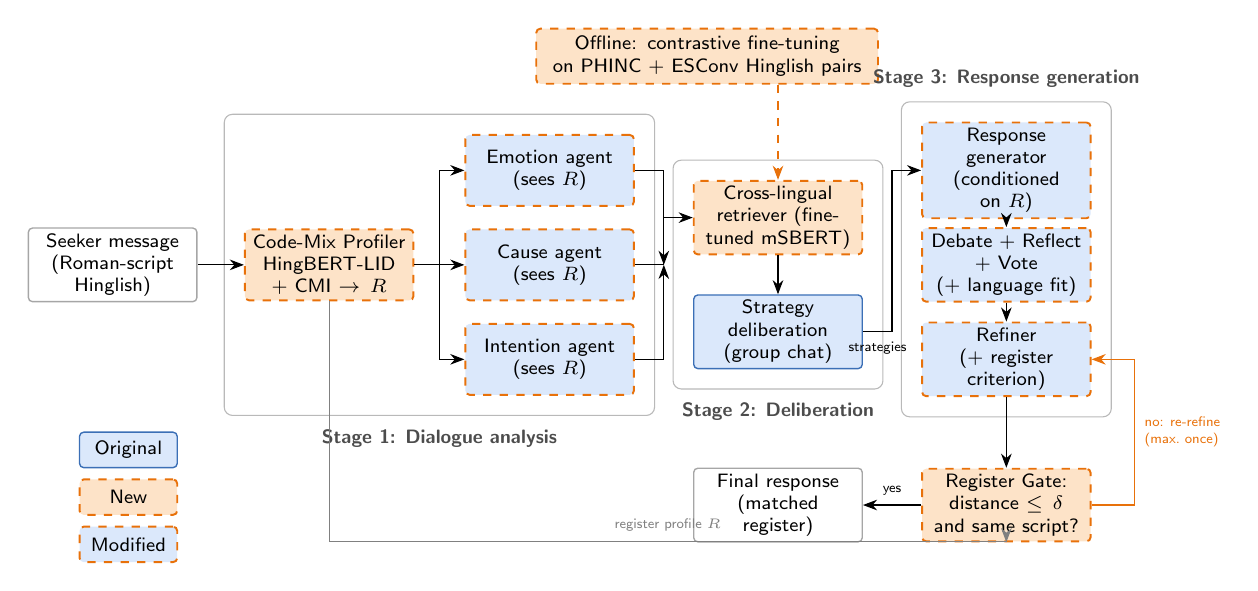
\begin{tikzpicture}[
  font=\scriptsize, >={Stealth[length=1.8mm]},
  box/.style={draw=origline, fill=orig, rounded corners=1.5pt, align=center, minimum height=9mm,
              text width=20mm, line width=0.5pt, inner sep=2pt},
  new/.style={box, draw=newline, fill=new, dashed, line width=0.7pt},
  mod/.style={box, draw=newline, dashed, line width=0.7pt},
  io/.style={box, draw=gray!70, fill=white},
  stage/.style={draw=gray!55, rounded corners=3pt, inner sep=2.5mm},
  lab/.style={font=\scriptsize\bfseries, text=gray!60!black}]
% ---------------- nodes (absolute positions, cm)
\node[io]  (seek) at (0, 0)     {Seeker message\\(Roman-script\\Hinglish)};
\node[new] (prof) at (2.75, 0)  {Code-Mix Profiler\\HingBERT-LID\\+ CMI $\rightarrow R$};
\node[mod] (emo)  at (5.55, 1.2) {Emotion agent\\(sees $R$)};
\node[mod] (cau)  at (5.55, 0)   {Cause agent\\(sees $R$)};
\node[mod] (int)  at (5.55, -1.2) {Intention agent\\(sees $R$)};
\node[new] (ret)  at (8.45, 0.6)  {Cross-lingual\\retriever (fine-\\tuned mSBERT)};
\node[box] (del)  at (8.45, -0.85) {Strategy\\deliberation\\(group chat)};
\node[mod] (gen)  at (11.35, 1.2) {Response generator\\(conditioned\\on $R$)};
\node[mod] (deb)  at (11.35, 0)   {Debate + Reflect\\+ Vote\\(+ language fit)};
\node[mod] (ref)  at (11.35, -1.2) {Refiner\\(+ register\\criterion)};
\node[new] (gate) at (11.35, -3.05) {Register Gate:\\distance $\le\delta$\\and same script?};
\node[io]  (out)  at (8.45, -3.05) {Final response\\(matched\\register)};
\node[new, text width=42mm, minimum height=7mm] (train) at (7.55, 2.65)
      {Offline: contrastive fine-tuning\\on PHINC + \mbox{ESConv} Hinglish pairs};
% ---------------- stage frames
\begin{scope}[on background layer]
\node[stage, fit=(prof)(emo)(int)] (s1) {};
\node[stage, fit=(ret)(del)] (s2) {};
\node[stage, fit=(gen)(deb)(ref)] (s3) {};
\end{scope}
\node[lab, anchor=north] at ($(s1.south)+(0,-0.05)$) {Stage 1: Dialogue analysis};
\node[lab, anchor=north] at ($(s2.south)+(0,-0.05)$) {Stage 2: Deliberation};
\node[lab, anchor=south] at ($(s3.north)+(0,0.05)$) {Stage 3: Response generation};
% ---------------- edges
\draw[->] (seek) -- (prof);
\coordinate (j1) at ($(prof.east)!0.5!(cau.west)$);
\draw[->] (prof.east) -- (j1) |- (emo.west);
\draw[->] (j1) -- (cau.west);
\draw[->] (j1) |- (int.west);
\coordinate (j2) at ($(cau.east)!0.5!(ret.west|-cau.east)$);
\draw[->] (emo.east) -| (j2);
\draw[->] (int.east) -| (j2);
\draw (cau.east) -- (j2);
\draw[->] (j2) |- (ret.west);
\draw[->] (ret) -- (del);
\coordinate (j3) at ($(del.east)!0.5!(gen.west|-del.east)$);
\draw[->] (del.east) -- node[below, font=\tiny] {strategies} (j3) |- (gen.west);
\draw[->] (gen) -- (deb);
\draw[->] (deb) -- (ref);
\draw[->] (ref) -- (gate);
\draw[->] (gate) -- node[above, font=\tiny] {yes} (out);
\draw[->, newline] (gate.east) -- ++(0.55,0) |- node[pos=0.25, right, font=\tiny, align=left] {no: re-refine\\(max.\ once)} (ref.east);
\draw[->, dashed, newline] (train.south -| ret) -- (ret);
\draw[->, gray] (prof.south) -- ++(0,-3.05) -| node[pos=0.25, above, font=\tiny] {register profile $R$} (gate.south);
% ---------------- legend
\node[box, text width=11mm, minimum height=4.5mm] (l1) at (0.2, -2.35) {Original};
\node[new, text width=11mm, minimum height=4.5mm] (l2) at (0.2, -2.95) {New};
\node[mod, text width=11mm, minimum height=4.5mm] (l3) at (0.2, -3.55) {Modified};
\end{tikzpicture}
\end{document}
